%\tikzset{external/force remake}
\begin{frame}{The yoghurt creep experiment}
\tikzsetnextfilename{creep_spoon}
\begin{tikzpicture}
\node[anchor=south west] (webcam){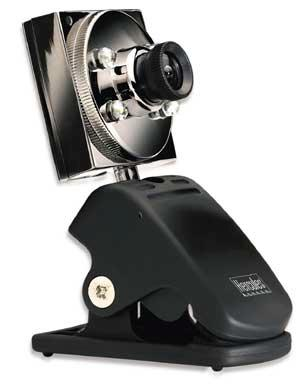
\includegraphics[width=0.2\textwidth]{webcam}};
\node[anchor=south] at (0.4\textwidth,0) (spoon) {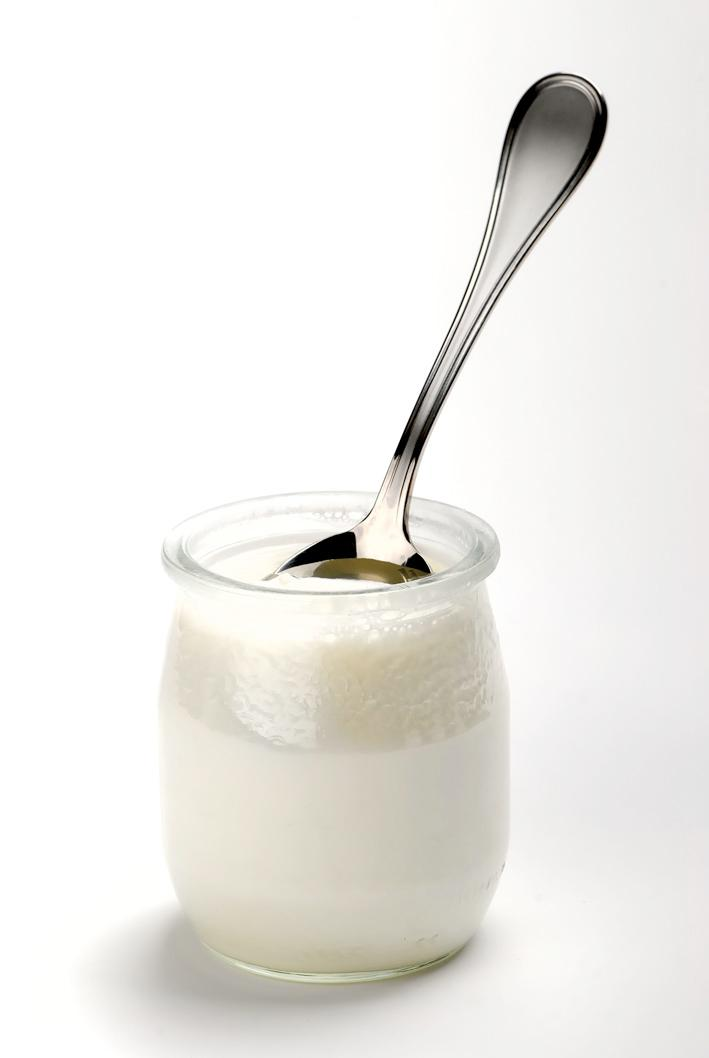
\includegraphics[width=0.3\textwidth]{spoon}};
\node[anchor=south east] at (\textwidth,0) (ultrasound) {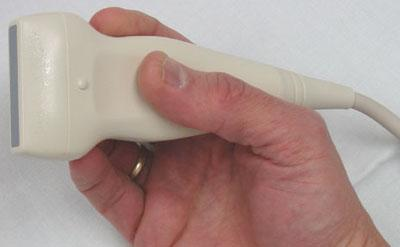
\includegraphics[width=0.4\textwidth]{ultrasound}};

\node[anchor=south west] at ($(ultrasound.north west)+(0,2em)$) (rheometer) {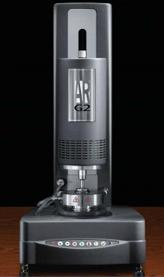
\includegraphics[height=0.4\textheight]{rheometer}};


%Couette cell
\let\mydimb\relax
	\newlength\mydimb
	\pgfmathsetlength{\mydimb}{6\baselineskip}

\node[shape=cylinder, draw, shape border rotate=90,minimum width=\mydimb, minimum height=7\baselineskip, anchor=north, aspect=2, yshift=-1.5em] at (rheometer.north-|webcam.north) (Stator) {};

\node[shape=cylinder, draw, shape border rotate=90,minimum width=\mydimb-1em, minimum height=6.75\baselineskip, anchor=before bottom , aspect=1.5] at ($(Stator.before bottom)+(-0.5em,0)$) (Rotor){};

\draw[->, x radius=0.5\mydimb-2em, y radius=0.2\baselineskip]  (Stator.before top) ++(0.5\mydimb,+0.2\baselineskip) arc[start angle=90, end angle=270] node[right=1mm, font=\scriptsize] {$\sigma$};

\begin{scope}[draw]
	\node[below right=0of Stator.north east, text width=0.2\textwidth, align=center] (couette) {A Taylor-Couette cell where the yogurt is made \emph{in situ}};
	\draw[->] ($(spoon.west)+(2em,0)$) -- (Stator);
	\node[below=0of ultrasound] {ultrasonic velocimetry};
	\node[below right=0of webcam.south west, text width=0.25\textwidth, align=center] {optical imaging};
	\draw[->] (spoon.north east) +(235:2em) -- (rheometer);
	\node[right=0of rheometer, text width=0.2\textwidth, align=center] {A rheometer imposes a constant stress $\sigma$ and records the strain $\gamma(t)$};
\end{scope}
\end{tikzpicture}
\end{frame}



\begin{frame}{The yoghurt creep experiment}
\vspace{1.25\baselineskip}
\let\mylena\relax
\newlength\mylena
\pgfmathsetlength{\mylena}{0.19\textwidth}
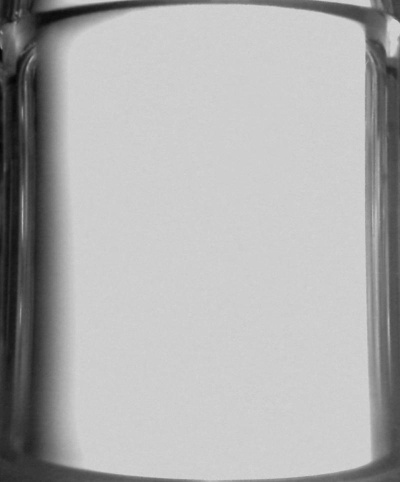
\includegraphics[width=\mylena]{Y110_2013-03-01_02-55-11.jpg}\hfill
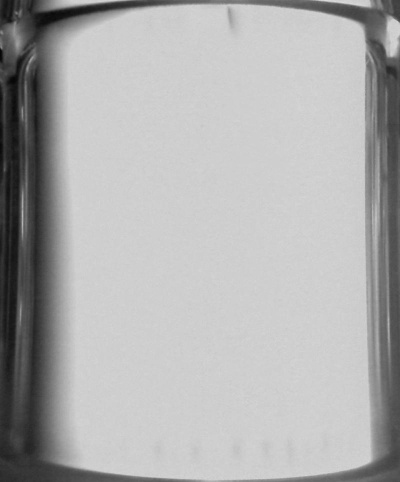
\includegraphics[width=\mylena]{Y110_2013-03-01_03-06-28.jpg}\hfill
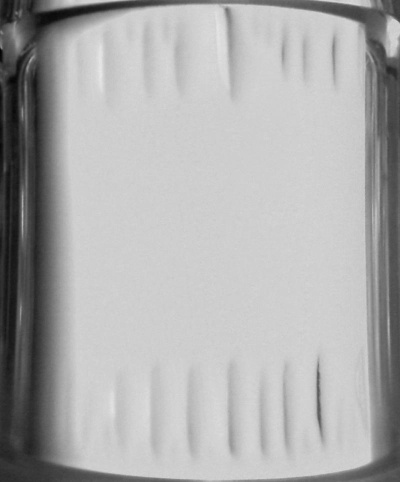
\includegraphics[width=\mylena]{Y110_2013-03-01_03-19-47.jpg}\hfill
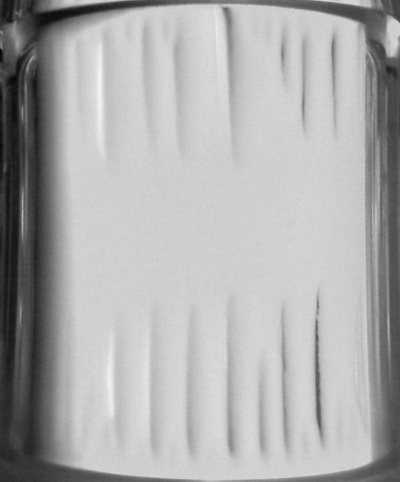
\includegraphics[width=\mylena]{Y110_2013-03-01_03-21-10.jpg}\hfill
%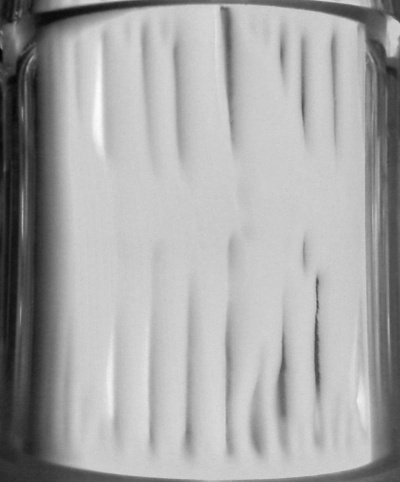
\includegraphics[width=\mylena]{Y110_2013-03-01_03-21-18.jpg}\hfill
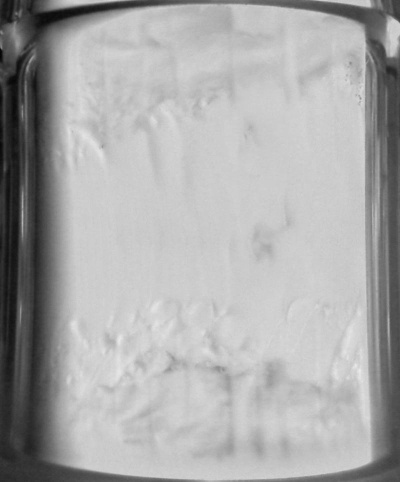
\includegraphics[width=\mylena]{Y110_2013-03-01_03-21-19.jpg}\\
%\begin{center}


\bigskip\tikzsetnextfilename{creep_xp_snapshot}
\begin{tikzpicture}
\begin{axis}[
	width=\textwidth,
	height=12\baselineskip,
	xmode=log,
	ymode=log,
	xlabel={$t$ (\si{\second})},
	xmin=0.1,
	ylabel={strain rate $\dot\gamma$ (\si{\per\second})}, 
	ymin=0.9e-4, ymax=2e-1,
	axis on top,
	]
 	\fill[Accent1!20]
		(axis cs:3,1e-2) ellipse[rotate=-25, x radius=0.4\textwidth, y radius=0.04\textwidth] node[below, rotate=-25, black] {power-law creep}
		(axis cs:0.8e3,2e-4) ellipse[x radius=0.05\textwidth, y radius=0.02\textwidth] node[below, black] {nucleation}
		(axis cs:1577,1e-2) ellipse[x radius=0.04\textwidth, y radius=4\baselineskip] node[below, rotate=90, black] {explosive regime}
		;
	\addplot[thick] table {Y110_300Pa.gdot}; 
	\addplot[thick, only marks, mark=o] coordinates {(687, 2.1e-4) (1476, 7.35e-4) (1509, 1.12e-3)};
	\node[below] at (rel axis cs:0.5,1) {$\sigma=\SI{300}{\pascal}$};
\end{axis}
\end{tikzpicture}
\end{frame}

\begin{frame}{Different stresses: universality}
\begin{columns}
\column{0.4\textwidth}
\textit{\footnotesize constant stresses}\\
\vspace{\baselineskip}
\structure{Normalisation}
\begin{description}[$\dot\gamma_\text{min}$]
\item[$\tau_f$] failure time 
\item[$\dot\gamma_\mathrm{min}$] minimum strain rate 
\end{description}

\smallskip
\hfill\begin{beamercolorbox}[rounded=true]{block title}\Large $\Rightarrow$Physical origin?\end{beamercolorbox}

\column{0.6\textwidth}
\tikzsetnextfilename{gdots_not_normed}%
\begin{tikzpicture}
\begin{loglogaxis}[
	name=g,
	width=\textwidth,
	height=10\baselineskip,
	xmin=2e-2, xmax=4e5, xlabel={time (\si{\second})},
	ylabel={Strain rate $\dot{\gamma}$ (\si{\per\second})},
	cycle list name=earthy,
	no marks,
	]
% 	\fill[Accent1!20]
% 		(axis cs:10,0.4) ellipse[rotate=-20, x radius=0.15\textwidth, y radius=0.02\textwidth]
% 		(axis cs:2e2,1.6) ellipse[x radius=0.35\textwidth, y radius=0.05\textwidth]
% 		(axis cs:3e3,0.85) ellipse[rotate=-7.5, x radius=0.3\textwidth, y radius=0.07\textwidth]
% 		;
	\addplot table[y index=2]{Y27_200Pa_gdot_decimated.txt} node (s200){};
	\addplot table[y index=2]{Y38_300Pa_gdot_decimated.txt} node (s300){};
	\addplot table[y index=2]{Y25_400Pa_gdot_decimated.txt}  node (s400){};
	\addplot table[y index=2]{Y32_550Pa_gdot_decimated.txt}  node (s550){};
	\addplot table[y index=2]{Y39_1000Pa_gdot_decimated.txt} node (s1000){};
	%\addplot[Accent2, ultra thick, domain={0.1:1e3}] {0.01*x^(-0.85)} node[sloped, pos=0.75, below left] {Primary creep};
	
\end{loglogaxis}
\begin{scope}[anchor=base east, every node/.style={ rotate=90}]
	\node[red!40!black] at (s200 |- g.outer north) {\SI{200}{\pascal}};
	\node[red!60!black] at (s300 |- g.outer north) {300};
	\node[red!80!black] at (s400 |- g.outer north) {400};
	\node[red] at (s550 |- g.outer north) {550};
	\node[red!80!yellow] at (s1000 |- g.outer north) {1000};
\end{scope}
\end{tikzpicture}
\end{columns}

\tikzsetnextfilename{gdots_normed}%
\begin{tikzpicture}
	\begin{groupplot}[%
		group style={
			group name=g, group size=3 by 1,
			horizontal sep=3em,
			},
		width=0.35\textwidth,
		cycle list name=earthy,
		no marks,
		clip mode=individual,
		]
	\nextgroupplot[
		title={power-law creep},
		xmin=1e-5, xmax=2, xlabel={$t/\tau_f$},
		ylabel={$\dot{\gamma}/\dot{\gamma}_\text{min}$},
		xmode=log,ymode=log,
		xtick={1e-4, 1e-2, 1},
		]
		\addplot table[x index=1, y index=3]{Y27_200Pa_gdot_decimated.txt};
		\addplot table[x index=1, y index=3]{Y38_300Pa_gdot_decimated.txt};
		\addplot table[x index=1, y index=3]{Y25_400Pa_gdot_decimated.txt};
		\addplot table[x index=1, y index=3]{Y32_550Pa_gdot_decimated.txt};
		\addplot table[x index=1, y index=3]{Y39_1000Pa_gdot_decimated.txt};
		%\addplot[yellow, ultra thick, samples at={1e-5,1e-4, 1e-3,1e-2,0.1,0.2,0.3,0.4,0.5,0.6,0.7,0.8,0.9, 0.99, 0.999, 0.9999, 0.99999}] {0.378*x^(-0.85) + 0.187/(1-x)};
		
	\nextgroupplot[
		title={fracture nucleation},
		xmin=0, xmax=1, xlabel={$t/\tau_f$},
		ymin=0.5, ymax=4,
		restrict y to domain=0.5:10,
		]
		\addplot table[x index=1, y index=3]{Y27_200Pa_gdot_decimated.txt};
		\addplot table[x index=1, y index=3]{Y38_300Pa_gdot_decimated.txt};
		\addplot table[x index=1, y index=3]{Y25_400Pa_gdot_decimated.txt};
		\addplot table[x index=1, y index=3]{Y32_550Pa_gdot_decimated.txt};
		\addplot table[x index=1, y index=3]{Y39_1000Pa_gdot_decimated.txt};
		%\addplot[yellow, ultra thick, domain={0.01:0.99}] {0.378*x^(-0.85) + 0.187/(1-x)};
		
	\nextgroupplot[
		title={explosive regime},
		xmin=1e-5, xmax=2, xlabel={$(\tau_f-t)/\tau_f$},
		x dir=reverse,
		xmode=log,ymode=log,
		xtick={1e-4, 1e-2, 1},
	]
		\addplot table[x expr=1-\thisrowno{1}, y index=3]{Y27_200Pa_gdot_decimated.txt};
		\addplot table[x expr=1-\thisrowno{1}, y index=3]{Y38_300Pa_gdot_decimated.txt};
		\addplot table[x expr=1-\thisrowno{1}, y index=3]{Y25_400Pa_gdot_decimated.txt};
		\addplot table[x expr=1-\thisrowno{1}, y index=3]{Y32_550Pa_gdot_decimated.txt};
		\addplot table[x expr=1-\thisrowno{1}, y index=3]{Y39_1000Pa_gdot_decimated.txt};
		%\addplot[yellow, ultra thick, samples at={1e-5,1e-4, 1e-3,1e-2,0.1,0.2,0.3,0.4,0.5,0.6,0.7,0.8,0.9, 0.99, 0.999, 0.9999, 0.99999}] {0.378*(1-x)^(-0.85) + 0.187/x};
	\end{groupplot}
\end{tikzpicture}
\end{frame}

\begin{frame}{Power-law creep and plasticity}
\begin{block}{``Andrade'' creep (1910)}
\begin{itemize}
\item Power-law creep known in \alert{ductile solids} for over a century
\item Classically explained by disinclination dynamics in crystals
\item Recently explained by plastic events in glasses\\\hfill \textit{\footnotesize Miguel et al., PRL 2002}
\end{itemize}
\end{block}

Any plastic event in yoghurt?

\bigskip
\movie[externalviewer]{\structure{Ultrasound velocimetry}}{Yaourt110_primary.avi} $\Rightarrow$ local velocity maps\\\hfill\textit{\footnotesize T. Gallot et al., Rev. Sci. Instrum. 84, 045107 (2013)}
\begin{itemize}
	\item homogeneous \movie[externalviewer]{strain field}{Yaourt110_profils.avi} (no wall slip, no shear band)
	\item if present, plastic events are below our resolution {\small (a~few~\si{\micro\metre})}
\end{itemize}
\end{frame}




\begin{frame}{Is creep damaging the structure?}
\vspace{0.25\baselineskip}
\begin{itemize}
\item Stop creep much before ($\gamma<0.3$) fracture nucleation ($\gamma\approx 1$)
\item Let relax $\Rightarrow$ No complete recovery
\item Reset deformation and start again $\Rightarrow$  superimposable
\end{itemize}

\tikzsetnextfilename{recovery}
\begin{tikzpicture}
\begin{axis}[
	width=\textwidth,
	height=8\baselineskip,
	xlabel={time (\si{\hour})},
	ylabel={strain $\gamma$},
	xmin=-0.15, xmax=7.5, xtick={0, 1, ..., 7},
	axis background/.style={fill=white},
	]
	\addplot[black, no marks] table[x expr={\thisrowno{0}/3600}] {Y261_oscil_creep_recovery_100Pa_decimated.txt};
	\begin{scope}[<-,Main, inner sep=0]
	\draw (axis cs:0,0) -- +(1em,0) node[anchor=west]{$\sigma\leftarrow \SI{100}{\pascal}$};
	\draw (axis cs:1/6,0.2727007) -- +(1em,0) node[anchor=west]{$\sigma\leftarrow 0$};
	\draw (axis cs:2.388,0.0159) -- +(0,1em) node[anchor=base east]{$\gamma\leftarrow 0$};
	\end{scope}
\end{axis}
\end{tikzpicture}

\begin{itemize}
\item Undamaged structure\raisebox{-0.6\baselineskip}[0pt][0pt]{$\left.\rule{0pt}{1.\baselineskip}\right\}\Rightarrow\begin{array}{c}\text{Plasticity cannot explain}\\ \text{power law}\end{array}$}
\item Viscous dissipation
\end{itemize}
\end{frame}

\begin{frame}{Power-law creep as linear response}
\begin{columns}[T]
\column{0.45\textwidth}
\tikzsetnextfilename{linear_rheology}
\begin{tikzpicture}
\begin{loglogaxis}[
	name=a,
	height=0.8\textwidth,
	width=\textwidth,
	xlabel={Frequency (\si{\hertz})}, ylabel={\textcolor{Accent1}{$G^\prime$}, \textcolor{Accent2}{$G^{\prime\prime}$}(\si{\pascal})},
	domain={6e-2:70},
	ymin=10,
	]
	\addplot[Accent1, only marks, mark=*] table{freqsweep_Y265_cas4_GDL1.txt};
	\addplot[Accent2, only marks, mark=o] table[y=LossModulus]{freqsweep_Y265_cas4_GDL1.txt};
	\addplot[Main, no marks]{100*x^0.15}  node[midway, below=1em] {$G^\prime\sim G^{\prime\prime}\sim f^{0.15}$};
	
\end{loglogaxis}
\end{tikzpicture}
\[ \boxed{\sigma \propto  \gamma f^\alpha} \xrightarrow{\mathrm{Fourier}} \boxed{\sigma \propto \gamma t^{-\alpha}} \]
Constant $\sigma$
\[ \boxed{\gamma(t) \propto \sigma t^{\alpha}} \xrightarrow{\frac{d}{dt}} \boxed{\dot\gamma(t) \propto \sigma t^{\alpha-1}}\]

\column{0.55\textwidth}
\tikzsetnextfilename{primary_rescaled}
\begin{tikzpicture}
\begin{loglogaxis}[
	width=\textwidth,
	height=0.8\textwidth,
	xmin=1e-5, xmax=2, xlabel={$t/\tau_f$},
	ylabel={$\dot{\gamma}/\dot{\gamma}_\text{min}$},
	cycle list name=earthy,
	clip mode=individual,
	]
	\addplot table[x index=1, y index=3]{Y27_200Pa_gdot_decimated.txt} node (s200){};
	\addplot table[x index=1, y index=3]{Y38_300Pa_gdot_decimated.txt} node (s300){};
	\addplot table[x index=1, y index=3]{Y25_400Pa_gdot_decimated.txt}  node (s400){};
	\addplot table[x index=1, y index=3]{Y32_550Pa_gdot_decimated.txt}  node (s550){};
	\addplot table[x index=1, y index=3]{Y39_1000Pa_gdot_decimated.txt} node (s1000){};
	\addplot[yellow, ultra thick, domain={1e-4:0.1}] {0.378*x^(-0.85)} node[Accent2,pos=0.75, below left, font=\footnotesize] {$\frac{\dot{\gamma}(t)}{\dot{\gamma}_\text{min}}\sim \left(\frac{t}{\tau_f}\right)^{-0.85}$};
\end{loglogaxis}
\end{tikzpicture}

Power-law creep is 
\begin{itemize}
\item the linear regime of the material 
\item up to 100\% strain!
\item explained without plasticity
\end{itemize}
\end{columns}
\end{frame}




\begin{frame}{Explaining the explosive regime}
\begin{columns}[T]
\column{0.45\textwidth}

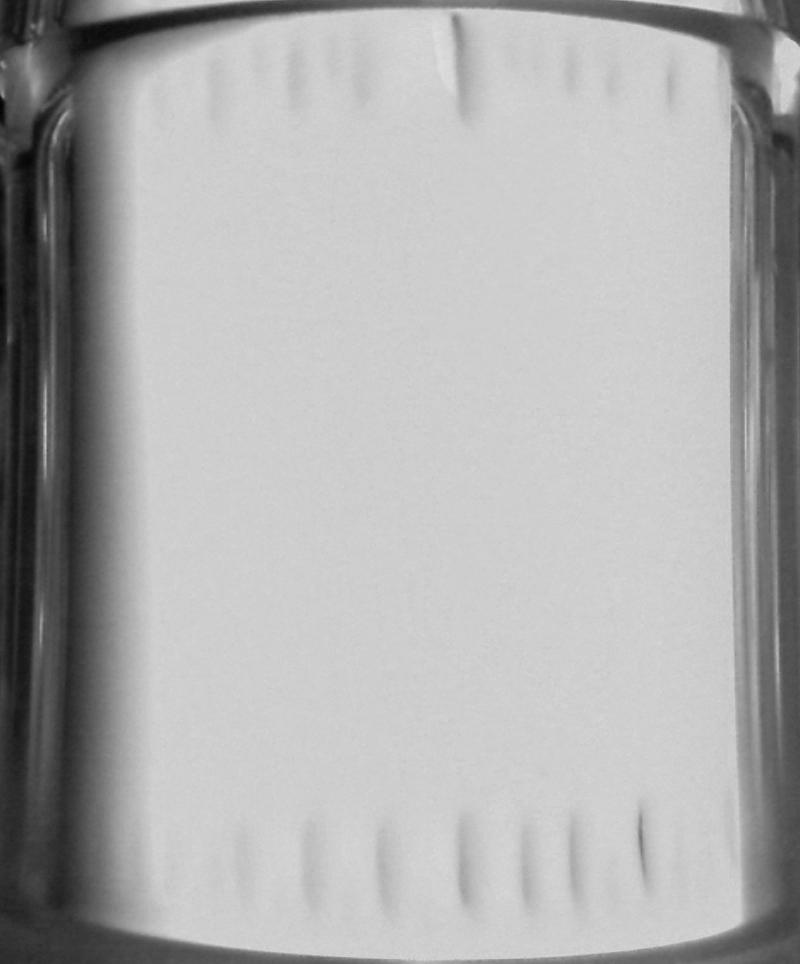
\includegraphics[width=0.33\textwidth]{Y110_2013-03-01_03-15-00.jpg}\hfill
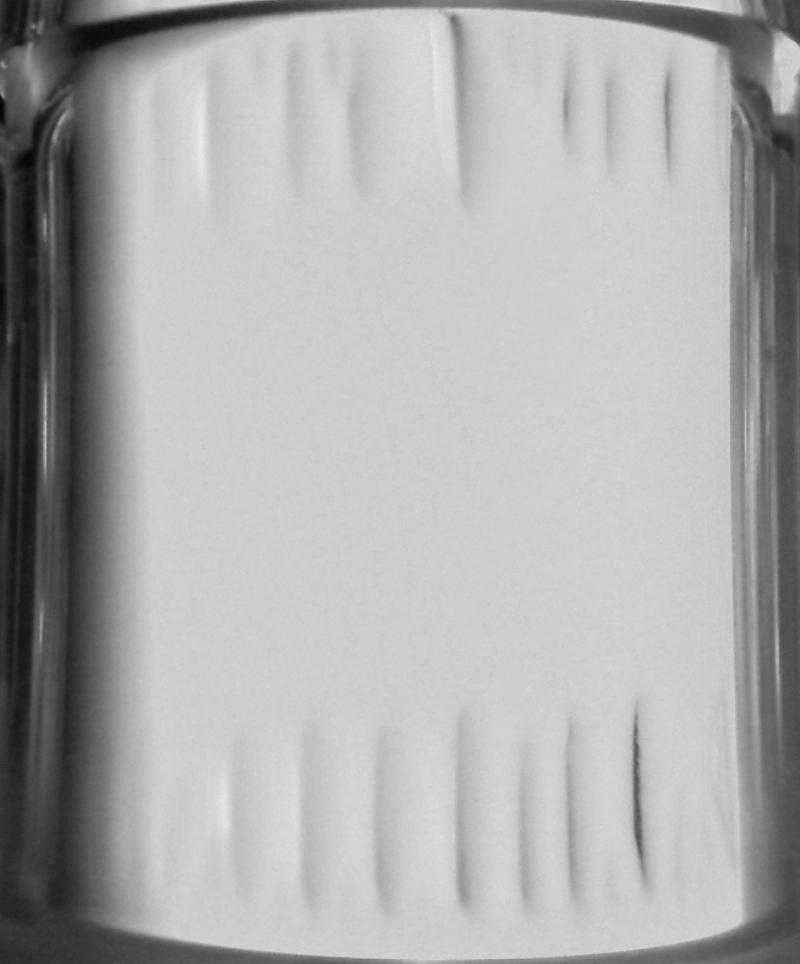
\includegraphics[width=0.33\textwidth]{Y110_2013-03-01_03-20-00.jpg}\hfill
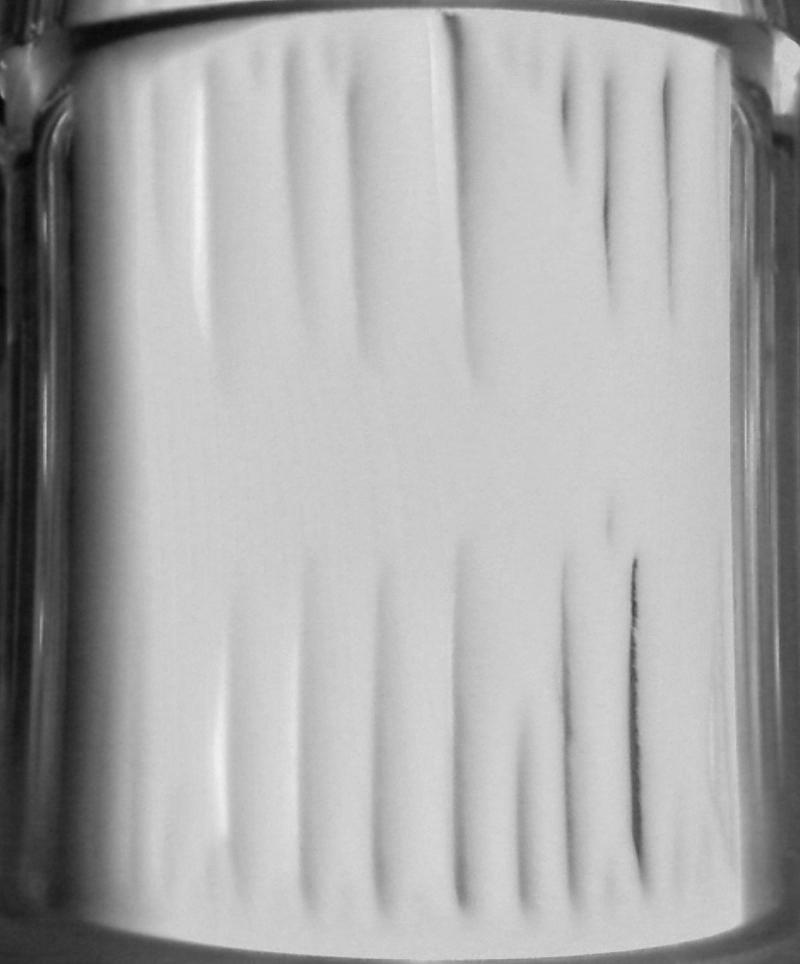
\includegraphics[width=0.33\textwidth]{Y110_2013-03-01_03-21-15.jpg}

\structure{Fracture length $\ell$}

\tikzsetnextfilename{fracture_length}
\begin{tikzpicture}
\begin{axis}[
	width=\textwidth,
	height=0.8\textwidth,
	xmin=1e-3, xmax=1, xlabel={$(\tau_f-t)/\tau_f$},
	xmode=log, x dir=reverse,
	ylabel={$\ell/H$},
	ymin=0, ymax=0.5,
	clip mode=individual,
	axis background/.style={fill=white},
	]
	\addplot[only marks, Accent1, error bars/.cd, y dir=both, y explicit] table[y error index=2]{Y110_fracturelength_log.txt};
	\addplot[Accent2, ultra thick, no marks, domain={1e-3:1}] {- 0.06 * ln(x)} node [pos=0.25,left=1em] {$\frac{\ell}{H}\sim \ln\frac{\tau_f-t}{\tau_f}$};
\end{axis}
\end{tikzpicture}

\column{0.55\textwidth}
\[ \gamma \propto \ell \propto \ln\frac{\tau_f-t}{\tau_f}\]

\[ \dot\gamma \propto \left(\frac{\tau_f-t}{\tau_f}\right)^{-1}\]

\tikzsetnextfilename{tertiary_rescaled}
\begin{tikzpicture}
\begin{loglogaxis}[
	width=\textwidth,
	height=0.8\textwidth,
	xmin=1e-5, xmax=2, xlabel={$(\tau_f-t)/\tau_f$},
	x dir=reverse,
	ylabel={$\dot{\gamma}/\dot{\gamma}_\text{min}$},
	cycle list name=earthy,
	clip mode=individual,
	]
	\addplot table[x expr=1-\thisrowno{1}, y index=3]{Y27_200Pa_gdot_decimated.txt} node (s200){};
	\addplot table[x expr=1-\thisrowno{1}, y index=3]{Y38_300Pa_gdot_decimated.txt} node (s300){};
	\addplot table[x expr=1-\thisrowno{1}, y index=3]{Y25_400Pa_gdot_decimated.txt}  node (s400){};
	\addplot table[x expr=1-\thisrowno{1}, y index=3]{Y32_550Pa_gdot_decimated.txt}  node (s550){};
	\addplot table[x expr=1-\thisrowno{1}, y index=3]{Y39_1000Pa_gdot_decimated.txt} node (s1000){};
	\addplot[yellow, ultra thick, domain={1e-4:0.1}] {0.187/x} node[Accent2, pos=0.6, below right, inner sep=0, yshift=-0.5em] {$\frac{\dot{\gamma}(t)}{\dot{\gamma}_\text{min}}\sim \left(\frac{\tau_f}{\tau_f-t}\right)$};
\end{loglogaxis}
\end{tikzpicture}
\end{columns}
$\Rightarrow$ Explosive regime dominated by fracture growth
\end{frame}

\begin{frame}{Failure time \& master curve}
\begin{columns}[T]
\column{0.5\textwidth}
\tikzsetnextfilename{basquin}
\begin{tikzpicture}
\begin{loglogaxis}[
	width=\textwidth,
	height=0.8\textwidth,
	xlabel={$\sigma$ (\si{\pascal})},
	ylabel={$\tau_f$ (\si{\second})},
	xmin=100, ymin=10, ymax=1e6,
	xtick={100, 200,..., 1000}, xticklabels={100, 200,,, 500,,,,, 1000},
	]
	\addplot[only marks, Accent1] table[y index=3]{creep_cas4_gdl1_MCR.txt};
	\addplot[no marks, black, domain={100:1000}] {4.2e17*x^(-5.45)} node [midway, above right] {$\tau_f\sim \sigma^{-5.5}$};
	\node[above right] at (rel axis cs:0,0){No yield stress!};
\end{loglogaxis}
\end{tikzpicture}

\begin{block}{Basquin law $\tau_f\sim \sigma^{-\beta}$}
\begin{itemize}
\item fatigue (oscillatory stress)
\item heterogeneous solids
\end{itemize}
\end{block}

\column{0.5\textwidth}
\tikzsetnextfilename{secondary_rescaled}
\begin{tikzpicture}
\begin{axis}[
	width=\textwidth,
	height=0.8\textwidth,
	xmin=0, xmax=1, xlabel={$t/\tau_f$}, xtick={0,0.2,...,1},
	ylabel={$\dot{\gamma}/\dot{\gamma}_\text{min}$},
	ymin=0.5, ymax=4,
	cycle list name=earthy,
	restrict y to domain=0.5:10,
	clip mode=individual,
	]
	\addplot table[x index=1, y index=3]{Y27_200Pa_gdot_decimated.txt} node (s200){};
	\addplot table[x index=1, y index=3]{Y38_300Pa_gdot_decimated.txt} node (s300){};
	\addplot table[x index=1, y index=3]{Y25_400Pa_gdot_decimated.txt}  node (s400){};
	\addplot table[x index=1, y index=3]{Y32_550Pa_gdot_decimated.txt}  node (s550){};
	\addplot table[x index=1, y index=3]{Y39_1000Pa_gdot_decimated.txt} node (s1000){};
	\addplot[yellow, ultra thick, domain={0.01:0.99}] {0.378*x^(-0.85) + 0.187/(1-x)};
	\draw[<-] (axis cs:0.56,1) -- +(0,1em) node[above] {$\tau_\text{min}$};
\end{axis}
\end{tikzpicture}

\structure{Master curve}
\[\frac{\dot{\gamma}(t)}{\dot{\gamma}_\text{min}} = \underbrace{\lambda \left(\frac{t}{\tau_f}\right)^{-0.85}}_\text{linear response} + \underbrace{\frac{\mu}{1 - t/\tau_f}}_\text{fractures}\]
$\Rightarrow$ no room for plasticity
\end{columns}
\end{frame}














\begin{frame}{Fibre bundle models}
	\vspace{\baselineskip}
	\tikzsetnextfilename{FBM_Jagla}%
	\begin{tikzpicture}
	\let\mydima\relax
	\newlength\mydima
	\setlength{\mydima}{0.3\textwidth}
	\let\mydimb\relax
	\newlength\mydimb
	\setlength{\mydimb}{2\baselineskip}
	
	\node[fill=black, inner sep=0, minimum height=0.2em, minimum width=\mydima] at (0,\mydimb)  (top) {};
	\node[fill=black, inner sep=0, minimum height=0.2em, minimum width=\mydima] at (0,-\mydimb)  (bot) {};
	
	\foreach \x in {0.1,0.2,...,0.9}\draw[Accent1, line width=0.1em*sin(1500*\x)+0.3em] (top.south west) ++(\x\mydima, 0) -- +(0, -2\mydimb+0.2em);
	
	\node[above=0 of top, single arrow, draw, shape border rotate=90] {$\sigma$};
	\node[starburst, draw=Accent2, inner sep=0pt,  minimum width=0.1\mydima, minimum height=0.5\mydimb, starburst point height=0.15em] at (-0.1\mydima,0) {};
		\node[double arrow,draw, anchor=west, text width=0.25\textwidth, align=center] at (0.5\mydima,-0.5\mydimb) (model) {\structure{model}};
	\node[above left=\baselineskip and 0of model.east, text width=0.35\textwidth, inner sep=0] {\begin{itemize}
		\item elastic fibres
		\item local yield strain
		\item local coupling
		\end{itemize}};
	\end{tikzpicture}
	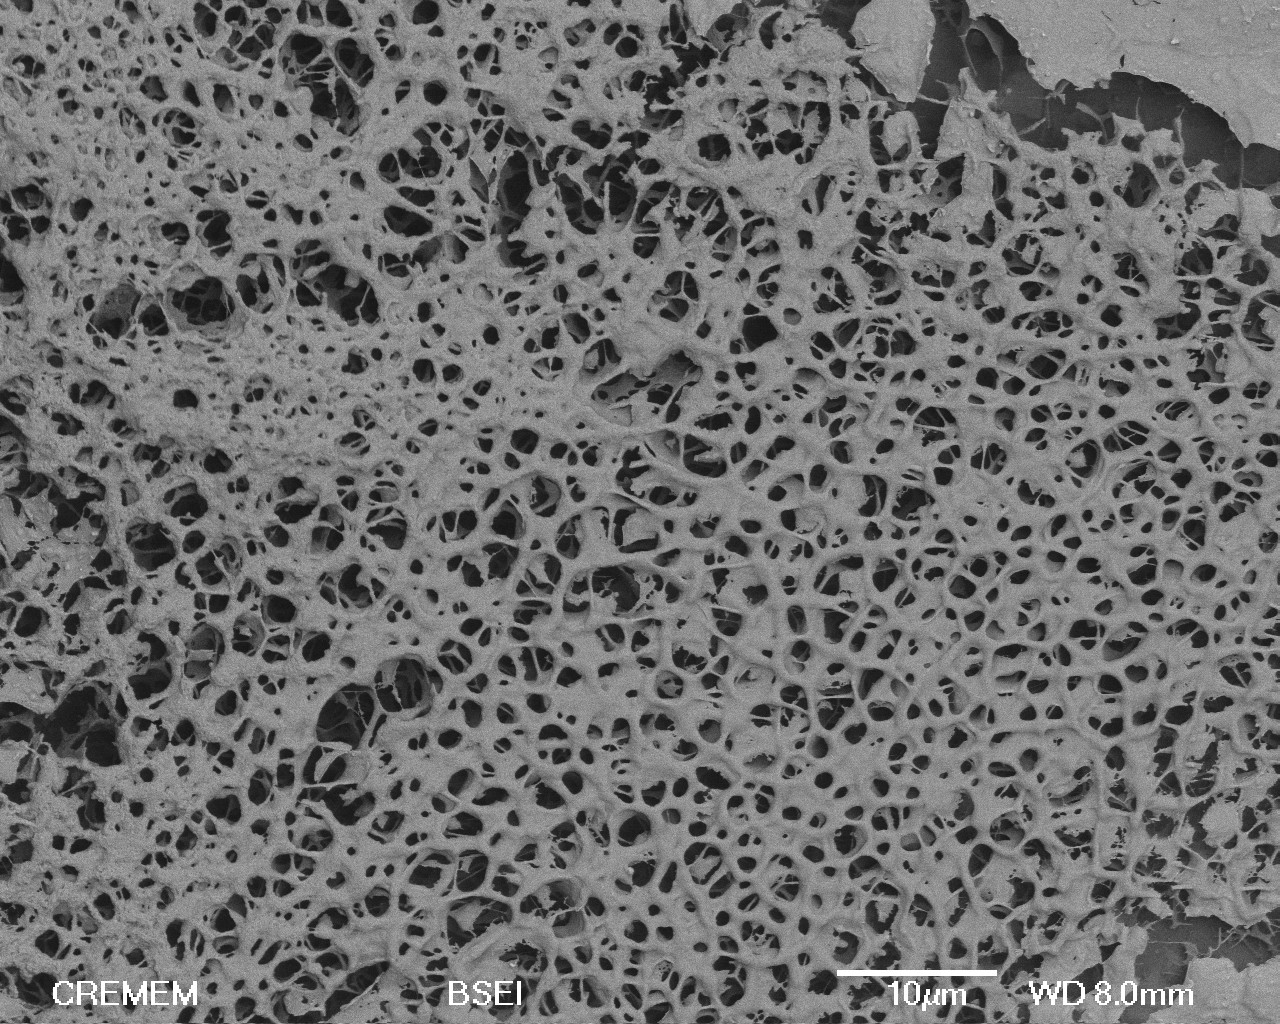
\includegraphics[width=0.35\textwidth, clip=true, trim=0 0 0 10cm]{MEB_cas4_gdl1_22}
	
	\bigskip
	\begin{columns}[b]
	\column{0.3\textwidth}
	\textit{\footnotesize Jagla et al., PRE 2011}
	
	\begin{minipage}[b][10\baselineskip][c]{1em}
	$\dot\gamma$
	
	\vspace{4\baselineskip}
	$\dot\gamma$
	\end{minipage}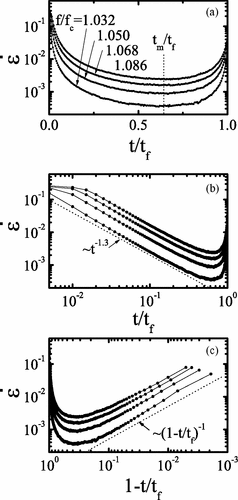
\includegraphics[height=10\baselineskip, clip=true, trim=7mm 0 0 6cm]{Jagla_2011_3regimes}
	
	\column{0.34\textwidth}
	\structure{But}
	\begin{itemize}
	\item yield stress
	\item built in power-law creep
	\item no master curve
	\end{itemize}
	
	\column{0.4\textwidth}\tikzsetnextfilename{creep_1_3}%
	\begin{tikzpicture}
		\begin{groupplot}[%
			group style={
				group name=g, group size=1 by 2,
				vertical sep=2.5em,
				},
			height=6.5\baselineskip,
			width=9\baselineskip,
			cycle list name=earthy,
			clip mode=individual,
			ylabel={$\dot{\gamma}/\dot{\gamma}_\text{min}$},
			xlabel shift=-0.5em,
			]
		\nextgroupplot[
			xmin=1e-5, xmax=2, xlabel={$t/\tau_f$},
			xmode=log,ymode=log,
			xtick={1e-4, 1e-2, 1},
			]
			\addplot table[x index=1, y index=3]{Y27_200Pa_gdot_decimated.txt};
			\addplot table[x index=1, y index=3]{Y38_300Pa_gdot_decimated.txt};
			\addplot table[x index=1, y index=3]{Y25_400Pa_gdot_decimated.txt};
			\addplot table[x index=1, y index=3]{Y32_550Pa_gdot_decimated.txt};
			\addplot table[x index=1, y index=3]{Y39_1000Pa_gdot_decimated.txt};
			\addplot[yellow, ultra thick, samples at={1e-5,1e-4, 1e-3,1e-2,0.1,0.2,0.3,0.4,0.5,0.6,0.7,0.8,0.9, 0.99, 0.999, 0.9999, 0.99999}] {0.378*x^(-0.85) + 0.187/(1-x)};
			
			
		\nextgroupplot[
			xmin=1e-5, xmax=2, xlabel={$(\tau_f-t)/\tau_f$},
			x dir=reverse,
			xmode=log,ymode=log,
			xtick={1e-4, 1e-2, 1},
		]
			\addplot table[x expr=1-\thisrowno{1}, y index=3]{Y27_200Pa_gdot_decimated.txt};
			\addplot table[x expr=1-\thisrowno{1}, y index=3]{Y38_300Pa_gdot_decimated.txt};
			\addplot table[x expr=1-\thisrowno{1}, y index=3]{Y25_400Pa_gdot_decimated.txt};
			\addplot table[x expr=1-\thisrowno{1}, y index=3]{Y32_550Pa_gdot_decimated.txt};
			\addplot table[x expr=1-\thisrowno{1}, y index=3]{Y39_1000Pa_gdot_decimated.txt};
			\addplot[yellow, ultra thick, samples at={1e-5,1e-4, 1e-3,1e-2,0.1,0.2,0.3,0.4,0.5,0.6,0.7,0.8,0.9, 0.99, 0.999, 0.9999, 0.99999}] {0.378*(1-x)^(-0.85) + 0.187/x};
		\end{groupplot}
	\end{tikzpicture}
	\end{columns}
\end{frame}


\begin{frame}{Fibre bundle models}
	\begin{columns}
	\column{0.27\textwidth}
	\vspace{0.5\baselineskip}
	\textit{\scriptsize Kun et al.  PRL 2008}
	
	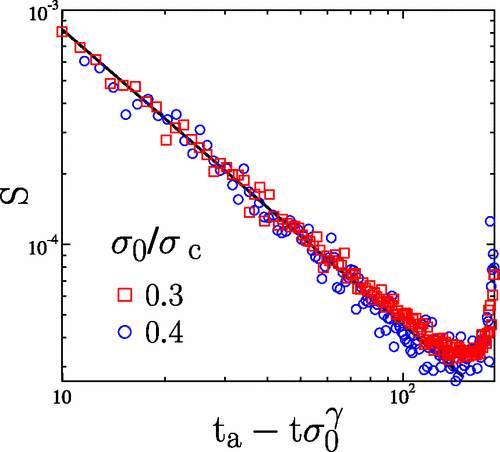
\includegraphics[height=6\baselineskip]{Kun_2008_Basquin}
	
	\textit{\scriptsize Halász et al. PRE 2012}
	
	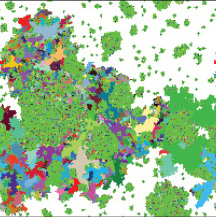
\includegraphics[height=6\baselineskip]{Halasz_2012_crack}
	
	\column{0.35\textwidth}
	\begin{itemize}
		\item elastic fibres
		\item local yield strain
		\item local coupling
		\item[+] damage accumulation
		\end{itemize}
	
	\tikzsetnextfilename{model_arrow}%
	\begin{tikzpicture}
	\node[double arrow,draw, anchor=west, text width=\textwidth-1\baselineskip, align=center] (model) {\structure{model}};
	\end{tikzpicture}
	
	\bigskip
	\structure{But}
	\begin{itemize}
	\item no power-law creep 
	\item too slow divergence
	\item 2D fractures
	\end{itemize}
	
	\column{0.38\textwidth}
	\tikzsetnextfilename{basquin_fracture}%
	\begin{tikzpicture}
	\begin{loglogaxis}[
		name=a,
		width=\textwidth,
		height=0.8\textwidth,
		xlabel={$\sigma$ (\si{\pascal})},
		ylabel={$\tau_f$ (\si{\second})},
		xmin=100, ymin=10, ymax=1e6,
		xtick={100, 200,..., 1000}, xticklabels={100, 200,,, 500,,,,, 1000},
		]
		\addplot[only marks, Accent1] table[y index=3]{creep_cas4_gdl1_MCR.txt};
		\addplot[no marks, black, domain={100:1000}] {4.2e17*x^(-5.45)};
	\end{loglogaxis}
	\node[below = of a]{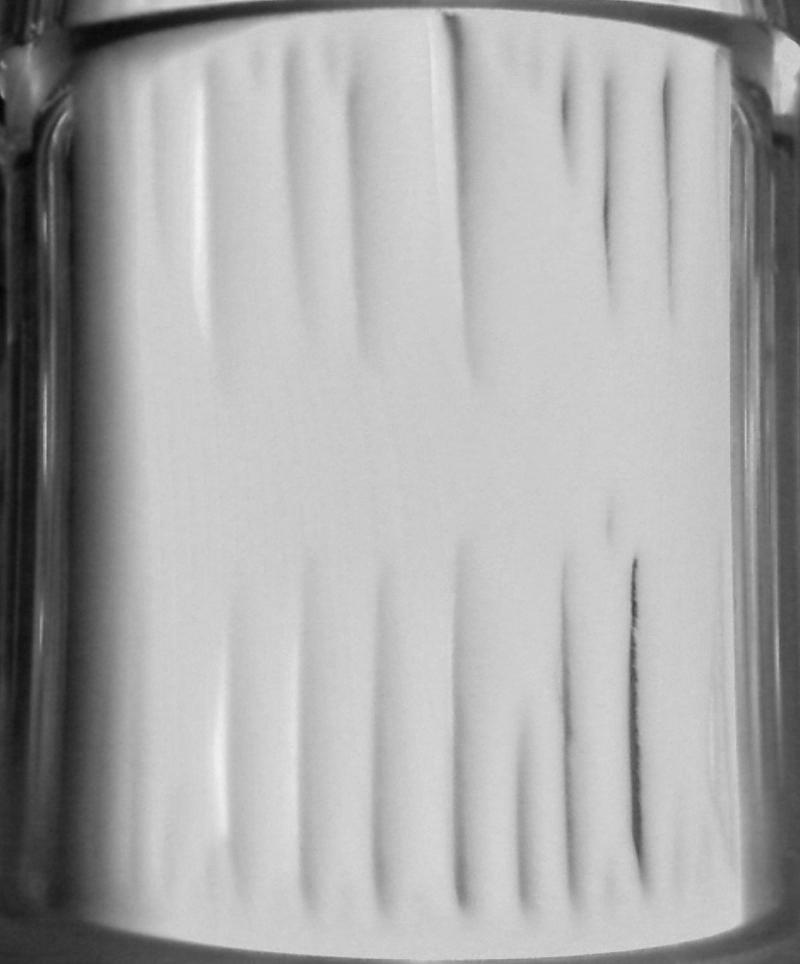
\includegraphics[height=6\baselineskip]{Y110_2013-03-01_03-21-15.jpg}};
	\end{tikzpicture}
	
	\end{columns}
\end{frame}

\begin{frame}{Creep and yielding summary}
\begin{itemize}
\item failure involves a single time scale $\tau_f \sim \sigma^{-5.5}$ Basquin law
\item $\left.\begin{minipage}{0.4\textwidth}\center reversible,\\ homogeneous creep\end{minipage}\right\rbrace$ \hfill\textcolor{ilmorange}{$\rightarrow$}\hfill $\left\lbrace\begin{minipage}{0.4\textwidth}\center irreversible fracture growth\end{minipage}\right.$
\item a single expression captures all the global rheological response
\end{itemize}
\tikzsetnextfilename{creep_summary}
\begin{tikzpicture}
	\begin{groupplot}[%
		group style={
			group name=g, group size=3 by 1,
			horizontal sep=2.5em,
			},
		width=0.375\textwidth,
		cycle list name=earthy,
		clip mode=individual,
		]
	\nextgroupplot[
		xmin=1e-5, xmax=2, xlabel={$t/\tau_f$},
		ylabel={$\dot{\gamma}/\dot{\gamma}_\text{min}$},
		xmode=log,ymode=log,
		xtick={1e-4, 1e-2, 1},
		]
		\addplot table[x index=1, y index=3]{Y27_200Pa_gdot_decimated.txt};
		\addplot table[x index=1, y index=3]{Y38_300Pa_gdot_decimated.txt};
		\addplot table[x index=1, y index=3]{Y25_400Pa_gdot_decimated.txt};
		\addplot table[x index=1, y index=3]{Y32_550Pa_gdot_decimated.txt};
		\addplot table[x index=1, y index=3]{Y39_1000Pa_gdot_decimated.txt};
		\addplot[yellow, ultra thick, samples at={1e-5,1e-4, 1e-3,1e-2,0.1,0.2,0.3,0.4,0.5,0.6,0.7,0.8,0.9, 0.99, 0.999, 0.9999, 0.99999}] {0.378*x^(-0.85) + 0.187/(1-x)};
		
	\nextgroupplot[
		xmin=0, xmax=1, xlabel={$t/\tau_f$},
		ymin=0.5, ymax=4,
		restrict y to domain=0.5:10,
		]
		\addplot table[x index=1, y index=3]{Y27_200Pa_gdot_decimated.txt};
		\addplot table[x index=1, y index=3]{Y38_300Pa_gdot_decimated.txt};
		\addplot table[x index=1, y index=3]{Y25_400Pa_gdot_decimated.txt};
		\addplot table[x index=1, y index=3]{Y32_550Pa_gdot_decimated.txt};
		\addplot table[x index=1, y index=3]{Y39_1000Pa_gdot_decimated.txt};
		\addplot[yellow, ultra thick, domain={0.01:0.99}] {0.378*x^(-0.85) + 0.187/(1-x)};
		
	\nextgroupplot[
		xmin=1e-5, xmax=2, xlabel={$(\tau_f-t)/\tau_f$},
		x dir=reverse,
		xmode=log,ymode=log,
		xtick={1e-4, 1e-2, 1},
	]
		\addplot table[x expr=1-\thisrowno{1}, y index=3]{Y27_200Pa_gdot_decimated.txt};
		\addplot table[x expr=1-\thisrowno{1}, y index=3]{Y38_300Pa_gdot_decimated.txt};
		\addplot table[x expr=1-\thisrowno{1}, y index=3]{Y25_400Pa_gdot_decimated.txt};
		\addplot table[x expr=1-\thisrowno{1}, y index=3]{Y32_550Pa_gdot_decimated.txt};
		\addplot table[x expr=1-\thisrowno{1}, y index=3]{Y39_1000Pa_gdot_decimated.txt};
		\addplot[yellow, ultra thick, samples at={1e-5,1e-4, 1e-3,1e-2,0.1,0.2,0.3,0.4,0.5,0.6,0.7,0.8,0.9, 0.99, 0.999, 0.9999, 0.99999}] {0.378*(1-x)^(-0.85) + 0.187/x};
	\end{groupplot}
\end{tikzpicture}
\begin{itemize}
\item a model soft solid well captured by fibre-bundle models
\end{itemize}
\end{frame}

